\documentclass[12pt]{article}
\usepackage{}
\usepackage[margin=2cm]{geometry}
\usepackage[authoryear,comma,round]{natbib}
\usepackage[separate-uncertainty=true,multi-part-units=single]{siunitx}
\usepackage{datatool,booktabs,hyperref,graphicx,caption,amsmath,amssymb}
\usepackage[list=true,listformat=simple]{subcaption}
\usepackage[para]{footmisc}
\usepackage[super]{nth}
\usepackage[utf8]{inputenc}

\DeclareSIUnit{\arcsec}{''}
\DeclareSIUnit{\au}{\mathrm{AU}}
\DeclareSIUnit{\mag}{\mathrm{mag}}
\DeclareSIUnit{\px}{\mathrm{px}}

\newcommand{\ttt}{\texttt}
\newcommand{\tess}{\textit{TESS}}
\newcommand{\tessellate}{\texttt{TESSELLATE}}
\newcommand{\red}[1]{\textcolor{red}{#1}}

\title{TESSELLATE asteroids paper}
\author{Brayden Leicester, Ryan Ridden-Harper, Michele Bannister and Others}
\begin{document}
\maketitle

\section{Abstract}\label{sec:Abs}
%TODO Later

% \twocolumn %To check size



\section{Introduction}\label{sec:Intro}

%TODO general opening statment about asteroids as transiet events/ moving objects

Since 2017, the Transiting Exoplanet Survey Satellite \citep[\tess,][]{Ricker2014} has been obseving large swathes ($\qty{96}{\degree}\times\qty{24}{\degree}$) of sky at a very high cadence.
These month long blocks of full frame images (FFIs) are named sectors, with the cadence of the sectors dependant on the cycle.
The cadence started at \qty{30}{\minute}, then increased to \qty{10}{\minute}, and has now increased again to \qty{200}{\second} FFIs.

The large archival dataset of \tess\ has gone largely unanalysed.
This is until the \tessellate\ project \defcitealias{TESSELLATE}{H. Roxburgh and R. Ridden-Harper et al. 2025}\citepalias{TESSELLATE}, which seeks to find all the transient events that were serendipitously observed by \tess.
\tessellate\ searches every pixel of every FFI from \tess, using the \ttt{TESSreduce} \citep{Ridden-Harper2021a} to looking for changes in brightness that could be related to a physical event.

Asteroids are the most numerous source of non-transient detections in \tessellate, and need to be filtered out of the rest of the data.
This also allows for analysis of the properties of these planetesimals.
This letter presents our analysis of the asteroids found with the third year of \tess\ sectors as analysed by \tessellate, with a \qty{10}{\minute} cadence. %?? Cite in prep something 
This cadence is fast enough that the Nyquist frequency of the observations is above the spin barrier for asteroids \citep{Pravec2000}, so \tess\ could detect new fast rotators.

There have been other studies done using \tess\ to characterise asteroids.
It was suggested by \citet{Pal2018} that it would be possible to get good photometry down to $V \lesssim \qty{19}{\mag}$.
They followed up with an analysis of the small bodies the first 12 sectors (cycle 1) \citep{Pal2020}, tripling the number of asteroids with accurate rotation periods.
\citet{McNeill2023} re-analyses the same sectors of cycle 1, and is in broad agreement with \citeauthor{Pal2020}.

As opposed to the population studies, single object analysis is also possible with \tess.
\citet{Humes2024} recover the period of an asteroid commensurate with Earth's rotation.
They also use the \tess\ data alongside other observations to determine the shape of the object.
\tess\ has been used to study comets as well \citep[e.g.][]{Ridden-Harper2021b}

\tess\ is used for solar-system observation in many other ways as well.
The Minor Planet Center (MPC) gets regular updates on asteroids in \tess\ from the \ttt{LINEAR-TESS} program \citep{Woods2021}.
\citet{Gowanlock2024} uses \tess\ photometry as well as observations by the Zwicky Transient Facility \citep[ZTF, ][]{Bellm2019} to get a longer baseline on mutually observed objects while combining ground and space-based observations.
Fainter and unknown solar system objects can be found by shift and stacking \citep{Holman2019, Payne2019, Rice2020} or taking a fast X-ray transform \citep{Nguyen2024} of the \tess\ FFI data.

For our analysis of the asteroids in \tess, we use the third year of observations from the spacecraft; sectors 27 to 39.
These were the first sectors to have a \qty{10}{\minute} cadence.
Our methods are presented in \autoref{sec:Meth}, followed by the results in \autoref{sec:Res}.
A discussion of how our results compare to other \tess\ asteroid studies is given in \autoref{sec:Dis}, and we conclude in \autoref{sec:Conc}.

\section{Methods}\label{sec:Meth}

%How they are found in TESSELLATE accidentally
\tessellate\ provides a new way to find and characterize asteroids: detecting them as transient events.
The lightcurves of these detections often have spike only a few frames long, as the asteroid moves over the pixel of interest.
Asteroids move at about \qty{1}{\px} per frame for the \qty{30}{\min} cadence \citep{Pal2018}, and thus are found as many different transient events as they cross a sector.
Both \ttt{SourceDetect} and \ttt{Starfind}, the detection methods employed by \tessellate, detect planetesimals.

Characterizing the spikes in the single pixel lightcurves as an ``asteroid'' has it's problems, as real transient events can look similar.
We have implemented another way of finding and removing asteroids from the set of detected events.
The reduction of full sectors during a \tessellate\ run also allows for forced photometry at known asteroid positions.
These can then be matched with the detections to classify the spikes, and properties of the asteroids can be measured at the same time.

%Conesearch w/ SkyBoT and names w/ Horizons
The position of known asteroids is important for matching them to detections.
We preform a conesearch with \ttt{SkyBoT} \citep{Berthier2006} to find all the asteroids with $V\leq \qty{20}{\mag}$, the limit suggested by \citep{Pal2018}.
We query every \qty{12}{\hour} over the month of the sector, and interpolate the positions to the times of the \tess\ observations.
With \tess's large pixel scale, these interpolations are accurate enough for our purposes, and save on time and resources, as the query can be expensive.
%? They were checked for accuracy against JPL Horizons

%Matching to TESSELLATE
The positions of these asteroids can be matched with the detections, using a KDTree \citep{Maneewongvatana1999}.
Setting boundaries of \qty{0.1}{\day} and \qty{1}{\px} %TODO check it is 1 px.
on the nearest match keeps only objects that are coincident temporally and spatially.
If two such objects  match to the same detection, the shortest distance between the positions is taken.
The matched events are then classified as asteroids, so other analyses of the \tessellate data can filter them out.

%-Forced Photometry Lightcurve
Forced photometry along the tracks of the asteroids allows for the construction of lightcurves.
The differenced images are used for the forced photometry, as the objects are moving they are not dimmed by the differencing.
% The positions are readjusted to the center of mass (COM) of the object.
Aperture photometry, using \texttt{Photutils} \citep{Bradley2024}, is preformed at the centre of mass of the point spread function with a \qty{1.5}{\px} aperture, the standard size of an aperture in \tessellate.
The lightcurves are then sigma-clipped to $3\sigma$ from the mean remove background stellar contamination.

%Lomb-Scargle Periodogram
From their lightcurves, the rotation period of the object can be determined by using a Lomb-Scargle periodogram \citep[\citet{Lomb1976, Scargle1982}, but see][ for a review]{VanderPlas2018}.
The new \ttt{NIFTY-LS} package \citep{Garrison2024},  as implemented in \ttt{astropy} \citep{Astropy2013,Astropy2018,Astropy2022}, was used to calculate the periodogram.
The periodogram searched for rotation periods between the Nyquist limit of \qty{20}{\minute} and a maximum of \qty{17}{\day} \citep[the value used in][ due to the length of the lightcurve]{McNeill2023}.
The uncertainty in the frequency is calculated as half full width half maximum of the peak found in the periodogram, crudely approximating the peaks as Gaussian.

%Example figure
\begin{figure}[!t]
    \centering
    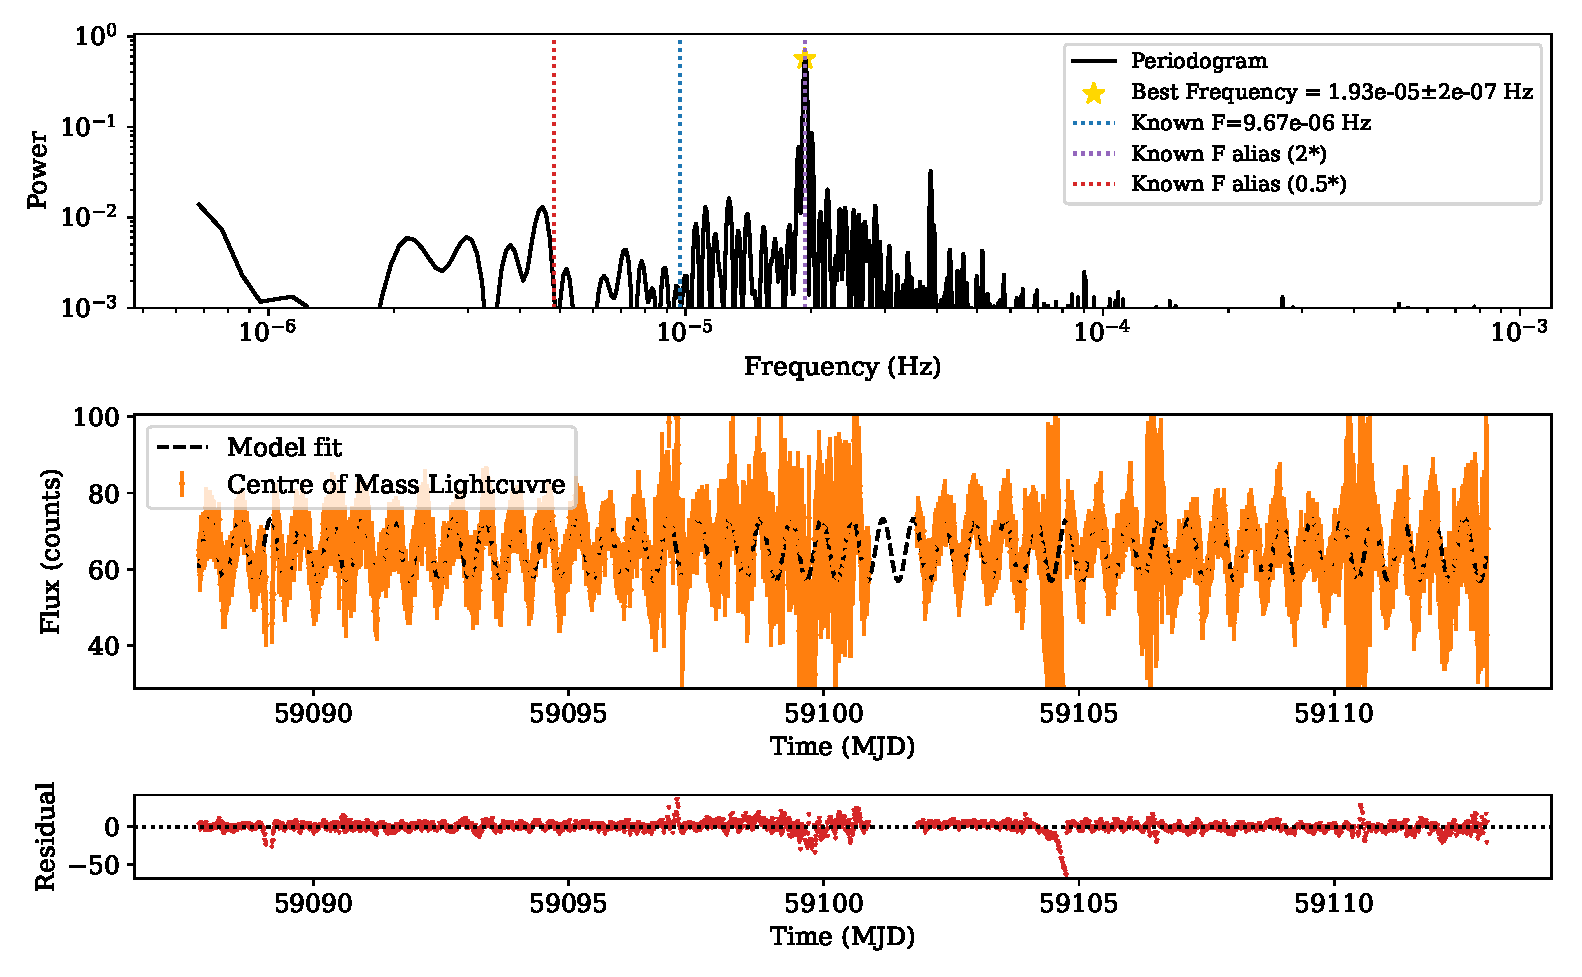
\includegraphics[width=\textwidth]{PeriodogramUlyssesPaperFigDraft.pdf}
    \caption{An example of the periodogram analysis we conduct for each object.
        This figure uses the lightcurve of the asteroid (5254) Ulysses from sector 29.
        Top panel: A periodogram of the lightcurve, with the known frequency and aliases indicated (from the LCDB).
        Middle panel: The lightcurve (orange error bars) and model(dashed black).
        Lower panel: Residuals of the difference between the model and the lightcurve.}
    \label{fig:perEx}
\end{figure}

An example of the periodogram fit to the lightcurve is given by \autoref{fig:perEx}.
A clear maximum power is found in the top panel, and the associated frequency is fed to the model shown in the middle panel.
The residuals in the lower panel are small for the most part, with large deviations from zero only where the lightcurve has large uncertainty in its flux.
Thanks to the known frequency from LCDB plotted, we note that we recover the double frequency alias, this is explored further below.

%Quality Checks on the lightcurves
Not every lightcurve is good enough for analysis, so some quality cuts are applied to them.
A minimum brightness cut of 10 counts ($m_T \sim \qty{18}{mag}$) %?which way around is better? 
is applied, otherwise the lightcurve is indistinguishable from noise. %* This is emperical from match to LCDB, should that fig be here?
%! No, fits the flow better in Results
This check is implemented to gain a better agreement when comparing to the known periods of these objects from the LCDB (elaborated on below).
Following \citeauthor{McNeill2023}, we do not trust the periods of any lightcurve with $\leq 200$ data points.

There were also quality cuts applied to the periodograms.
The methods would return the \qty{17}{\day} maximum value if no physical period was detected, so also following \citet{McNeill2023} we discard any periods within \qty{10}{\percent} of this maximum. 
\citet{McNeill2023} find that periods of $\leq \qty{3}{\hour}$ is also unreliable.
We are using data with a factor of three higher cadence, so we reduce this condition to $\leq \qty{1}{\hour}$ for the same number of observations sampled per rotation.
%// ! This and the doubling of the periods means we can't get fast rotators at all. Need to think this through
%* Addressed later


%-Run all these are part of TESSELLATE
The above methods are integrated into the rest of the \tessellate\ pipeline. %*I should probably get around to doing that...
This allows for asteroids to be filtered out of the new detections as they happen.
The results given below will be improved upon as more sectors are run and a higher number of minor planets can have their rotation properties measured.


\section{Results}\label{sec:Res}

%TODO Total Asteroids found

\red{57426} of asteroids with $V\leq \qty{20}{\mag}$ were found in the year 3 sectors we analysed.
Most of these are too faint for the lightcurve to give a reliable and period, while \citet{Pal2018} thinks good photometry down to $V\lesssim \qty{19}{\mag}$ should be achievable, we find the limit for \tessellate\ is closer to $m_{T} \approx \qty{17}{\mag}$ \citepalias{TESSELLATE}.
Once the quality checks (described above) have been applied, we are left with \red{4328} of planetesimals with accurate rotation rates. %!check double ups, I think this might drop to 4314
\red{\qty{80}{\percent}} of these asteroids do not have reliable periods reported in the LCDB, %TODO check defind before
so we are the first to get the rotation period for these bodies.


%TODO Properties of those that pass
%? TODO table of asteroids by class and frac that pass.


%TODO comp to LCDB
\begin{figure}
    \centering
    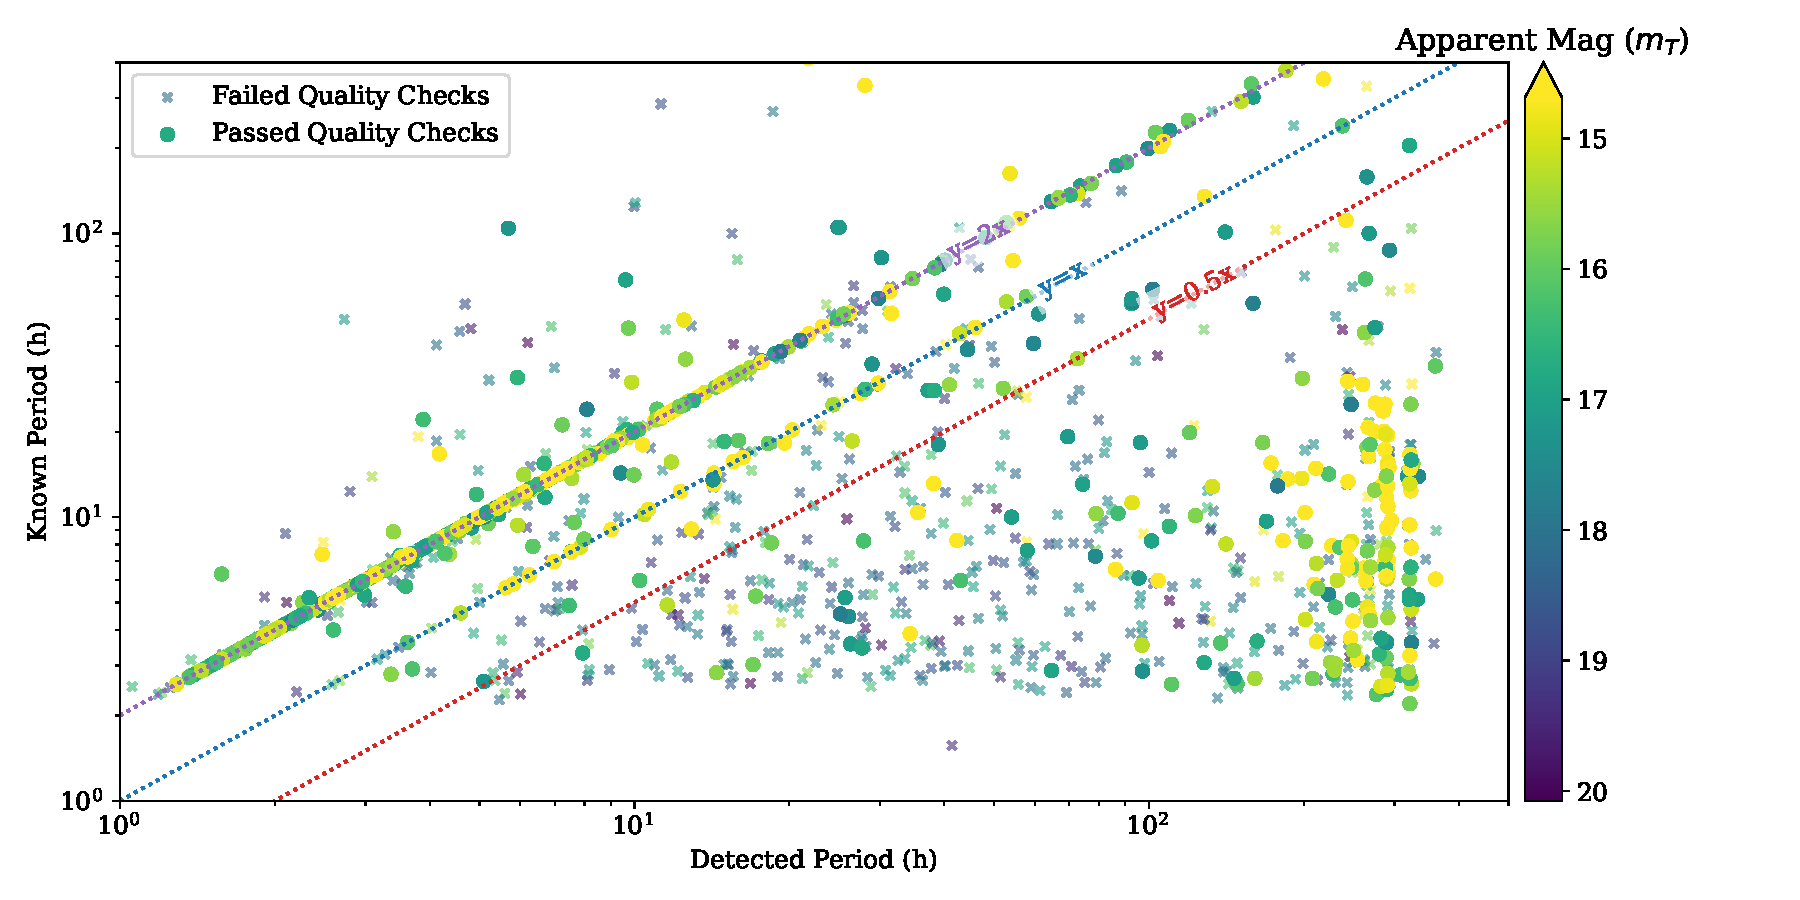
\includegraphics[width=\textwidth]{LCDBCompTotalPaperFigDraft.pdf}
    \caption{Comparison of the detected period and known period for all the asteroids analysed that are in the LCDB.
        Those that failed the quality check are shown with crosses, and those that passed are filled circles. They are coloured by the measured mean \tess\ magnitude ($m_T$).
        The 1:1 correspondence line (blue), and the factor of two aliases (purple ($\times 2$) and red ($\times 0.5$)) are plotted as dotted lines.
    }
    \label{fig:LCDBComp}
\end{figure}

%\red{57426 total, 1530 in LCDB, 868 of those pass check, 581 within 5 percent of y=2x, 28 within 5 percent of y=x}

We find \red{1530} of our total population of asteroids are in the LCDB with reliable periods. 
A comparison to our detected periods is given in \autoref{fig:LCDBComp}, and \red{868} asteroids pass the quality checks we describe above. 
The majority of these (\red{581} planetesimals) lie within \qty{5}{\percent} of the $y=2x$ line, indicating a double peaked lightcurve.
Only \red{28} objects have periods in direct agreement to the LCDB, far more of them are in disagreement. 
Most of the disagreement comes from systematically higher periods detected, and we are not sure why the known period is not found. 

%// TODO say we think only 70% are accurate. 
Following this comparison, we present double the periods we detect from periodograms as the rotation rate of these objects.
This is because $\approx \qty{70}{\percent}$ of the asteroid that pass the quality checks in \autoref{fig:LCDBComp} line within \qty{5}{\percent} of the $y=2x$ line; they have double peaked lightcurves.
A few percent have the same period detected as in the LCDB, but a larger fraction have periods detected with no relation to their known period.
Extrapolating this trend to the \red{4328} asteroids that pass the checks, we present an accurate rotation period for $\sim \red{3030}$ of them (unfortunately we cannot say which ones).

%// TODO justify 5% val.
We use an absolute difference between periods of $\leq\qty{5}{\percent}$ of our period as the agreement factor for a few reasons.
Direct agreement is tricky, floating point values and how precise they are presented varies between datasets, so exact equality is rare.
We did not want to have a set length of time to be the cut-off, as this would bias agreement to short periods. 
We are comparing to multiple datasets, the LCDB here and later \citet{McNeill2023} and \citet{Pal2020}, so we use \qty{5}{\percent} of our value for consistency.    

The brightness of the object during the observation seems to be the main factor for the passing of the quality checks.
We do apply a minimum brightness cut $(m_T \lesssim \qty{18}{\mag})$, there are plenty of objects with average $m_T$ between \nth{17} and \nth{18}\unit{\mag} in \autoref{fig:LCDBComp} that don't pass the other checks applied.
This is in agreement with the recovery rates of \tessellate\ at around \qty{17}{\mag} \citepalias{TESSELLATE}.
Raising the brightness cut we apply only removes some of the agreement with the LCDB, it doesn't drop the number of objects that pass the checks with periods far too large. 

\section{Discussion} \label{sec:Dis}

%TODO Comp to Pal and McNeill

Both \citet{Pal2020} and \citet{McNeill2023} published tables of the rotation properties for their asteroids.
For those objects we have in common, we compare the periods we find in \autoref{fig:otherWorksComp}.
There is good agreement in both cases, but our longer period detections haunt us here too. 

For \citet{McNeill2023}, the left panel of \autoref{fig:otherWorksComp}, we agree (to within \qty{5}{\percent} of our derived period) on \red{45} of the \red{139} objects. 
These are the asteroids that lie on the dotted $y=x$ line, and are close to one third of the asteroids.
They find higher periods for about a third of the asteroids, and then our incorrect high periods make the last third.

We find a higher agreement with \citet{Pal2020}, \red{63} of \red{117} objects within the \qty{5}{\percent} limits. 
So over half of our measurements agree with theirs, which is intriguing as our methods followed \citet{McNeill2023} more closely.
Most of the disagreement comes from out high period scatter and the systematic lower period found by \citet{Pal2020}. 

There are \red{54} asteroids in both all three datasets. 
\red{37} of them lie close to the $y=x$ line in the right \citeauthor{Pal2020} panel of \autoref{fig:otherWorksComp}, while only \red{14} agree with the measurements of \citeauthor{McNeill2023}. 
There are an extra \red{5} objects that \citet{Pal2020} and \citet{McNeill2023} find similar periods for, but we calculate a different period. 

\begin{figure}
    \centering
    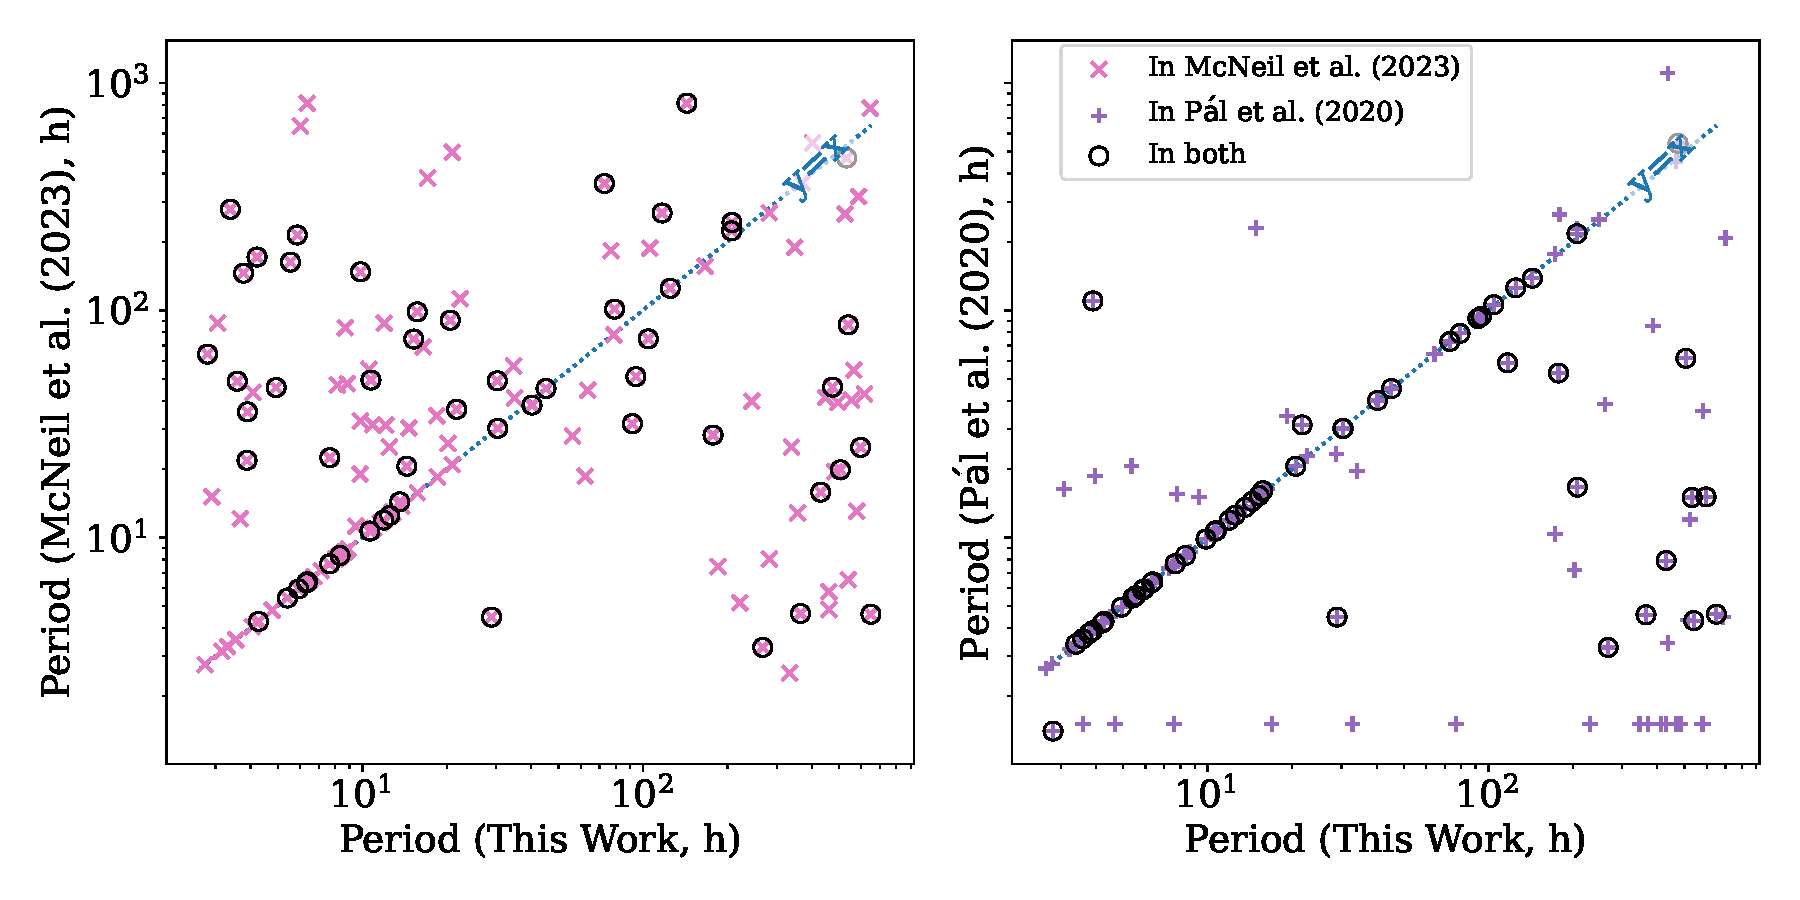
\includegraphics[width=\textwidth]{M23andP20CompPaperFigDraft.pdf}
    \caption{Comparing the rotation period of asteroids found in this work to asteroids in other studies that used TESS to investigate asteroids.
        Left: The comparison to \citet{McNeill2023} plotted as pink crosses, there are \red{139} objects.
        Right: The comparison to \citet{Pal2020} plotted as purple pluses, there are \red{117} objects.
        Those planetesimals found in all three works are circled (\red{54} asteroids).
        Lines of 1:1 agreement are plotted (dotted blue).}
    \label{fig:otherWorksComp}
\end{figure}


%TODO Fast Rotator Plot and discussion

\begin{figure}
    \centering
    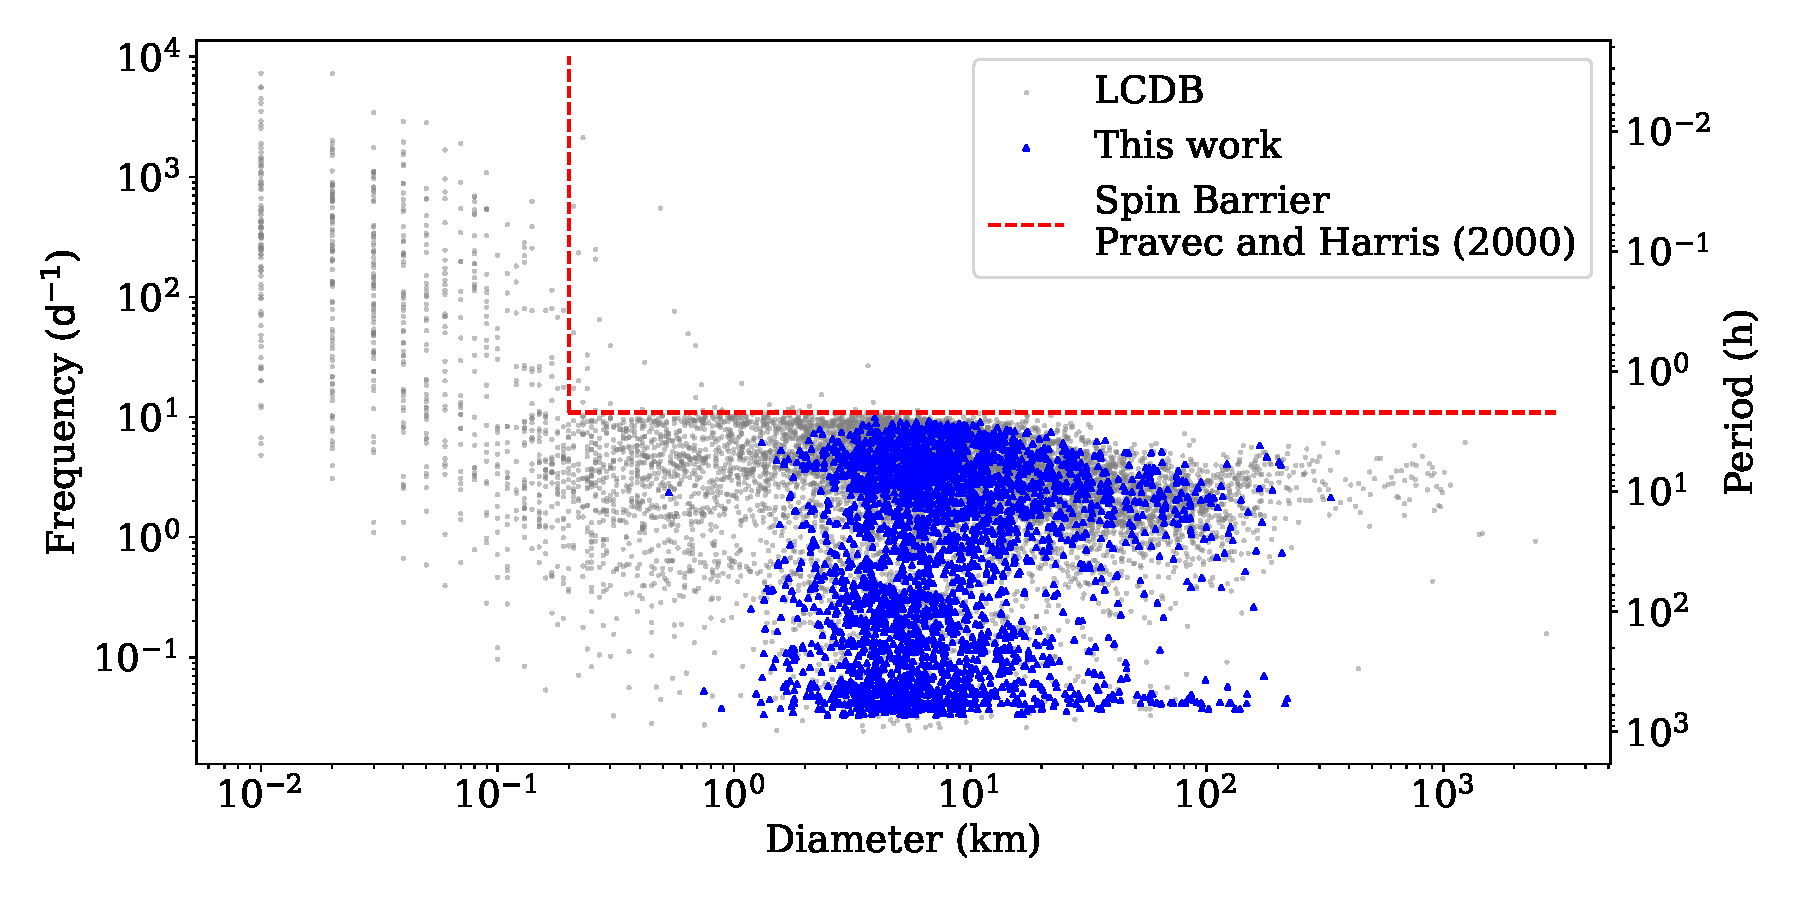
\includegraphics[width=\textwidth]{Diam-FreqPlotThisWorkPaperFigDraft.pdf}
    \caption{A rotation rate against size plot after the LCDB \citep{Warner2009} (grey
        circles) with this work's addition (blue squares). The
        diameters are from NEOWISE \citep{Masiero2011,NEOWISE2019} where available. The red dashed lines represent the spin barrier of \citep{Pravec2000}.}
    \label{fig:FreqDiam}
\end{figure}


We do not find any fast rotators in our dataset.
This is encapsulated by none of our objects being above the spin barrier shown in \autoref{fig:FreqDiam}.
While our Nyquist limit is well above the spin barrier of \citet{Pravec2000} thanks to \tess's fast cadence, most asteroids discovered above the barrier are small%? TODO CITE Warner2009 LCDB?
, and therefore dim.
The shallow magnitude of \tessellate\ \citepalias{TESSELLATE} makes it difficult for dim planetesimals to pass the quality checks.

%! we also can't actually go below 2hrs even with a 10 min cadence because we double the period.
Our presented periods could never be above the spin barrier, due to the minimum period quality check. 
We individually examine the \red{4} objects that pass the other checks, but have a period detected of less than an hour, and it is clear that the check is required.
\red{3} three of the objects have known periods in the LCDB, 2 of these are much longer than those we detect, and for the \red{\nth{3}} we find the $\times 4$ alias, instead of the usual $\times 2$.
The quality of the lightcurves of these objects is bad, they have large gaps and the fluxes vary wildly, even with the sigma-clipping done to them.

Through this extra analysis, we trust the quality cuts we have made even more. 
Unfortunately, this does mean we do not find any fast rotators.
The fast cadence of \tess\ and the multi-sector search with \tessellate\ were not enough to overcome the low data quality and the rarity of these objects.   

%TODO other discussion

The rotation periods of the brightest asteroids are not recovered.
This is due to the fixed aperture size of our forced photometry, \qty{1.5}{\px}.
The bright asteroids can start to saturate the \tess\ detector, and can bloom out to occupy more pixels.
We chose to keep a constant aperture to standardise the analysis, and to be agnostic to the properties of the asteroid being analysed.

Some asteroids slip through our detection methods, and end up unclassified in the \tessellate\ data.
This is often because the detections of bright asteroids are offset from the predicted positions by further than the matching radius we set.
Asteroids are easy to spot for our Cosmic Cataclysms \ttt{Zooniverse}\footnote{\url{https://www.zooniverse.org/projects/cheerfuluser/cosmic-cataclysms}} volunteers, as they are at a different position in the ``1 hour later'' panel, so any that slip past can be caught there.

%? TODO Why we detect long periods
%! I don't know. Ive tried supressing the exponetial that appears at low frequencies and adding the long cutoff. This kind of works, but only so much. 
%! Can't just take out anything we get above P=X hrs, as there are some slow rotators that we get correct. 

\section{Conclusion}\label{sec:Conc}
%TODO Later

%We find 43XX asteroids with good rotation properties

%Agree with McNeil and Pal in different amounts

%Do not find fast rotators

\bibliographystyle{aasjournal}
\bibliography{paperBib.bib}

\end{document}